\documentclass{beamer}
%\usepackage[latin1]{inputenc}
%\usepackage{lmodern}
\usepackage{times}
\usepackage[T1]{fontenc}
\usepackage{graphicx}
\usepackage{bm}
\usepackage{tikz}
\usepackage{verbatim}
\usepackage{amsmath}
\usepackage[small,labelformat=empty]{caption}
\usepackage{url}
\usetikzlibrary{automata,positioning}

\usetheme{Frankfurt}
%\usetheme{Warsaw}
\title[Title of presentation]{Uhrenbaustein\\
{\small Time&Date and Countdown}
}
\author[author name]
{Fabian Achatz}
\institute[Fnord GmbH]{Lehrstuhl f{\"u}r integrierte Systeme}
\date{Tue - 06/11/12}

\begin{document}

%{
%\usebackgroundtemplate{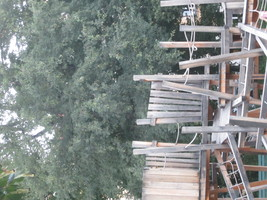
\includegraphics[width=\paperwidth]{pictures/sample.jpg}}
%\begin{frame}
%\thispagestyle{empty}
%\titlepage
%\end{frame}
%%}
%%
%\begin{frame}
%\frametitle{Overview}
%\tableofcontents
%\end{frame}
%
%\setlength\fboxsep{5pt}
%\setlength\fboxrule{0pt}




  \begin{frame}{Mode \_fsm Interface}  
  	\begin{figure}
  		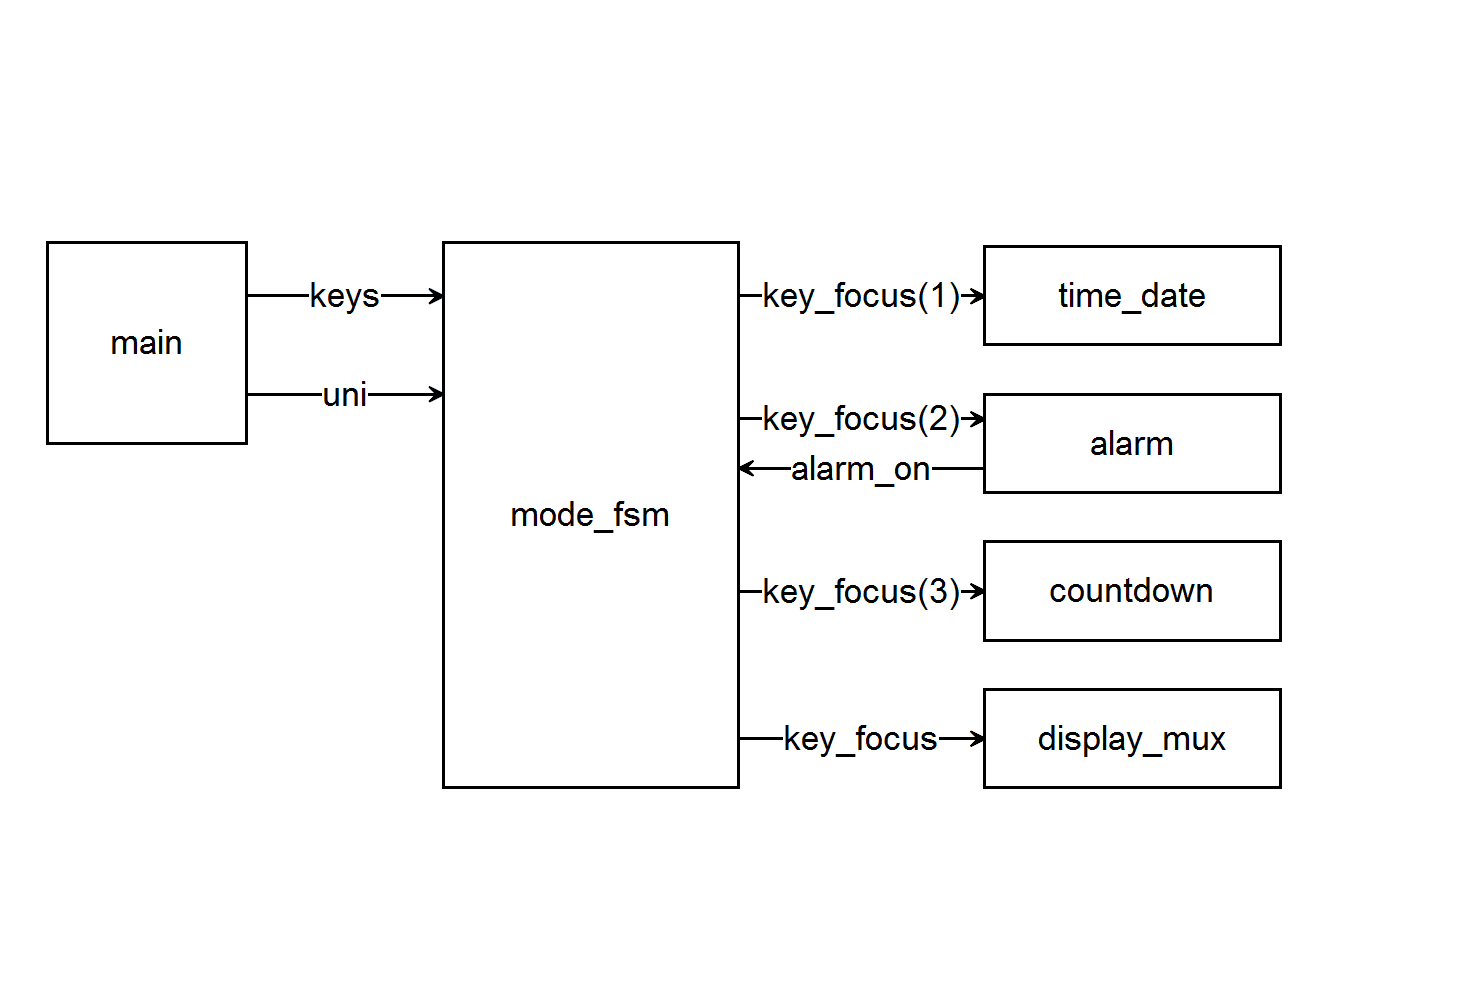
\includegraphics[width=100mm, height=70mm]{mode_fsm_interface.png}
  	\end{figure}
  \end{frame}
  
    \begin{frame}{Mode \_fsm Funktion}  
    	    \begin{itemize}
    	        \item Controls current mode
    	        \item Handles key access of modules (special case alarm ringing)
    	        \item Creates control signal for display\_mux
    	    \end {itemize}
    \end{frame}

  \begin{frame}{Mode \_fsm state diagram}
  	\begin{figure}
    	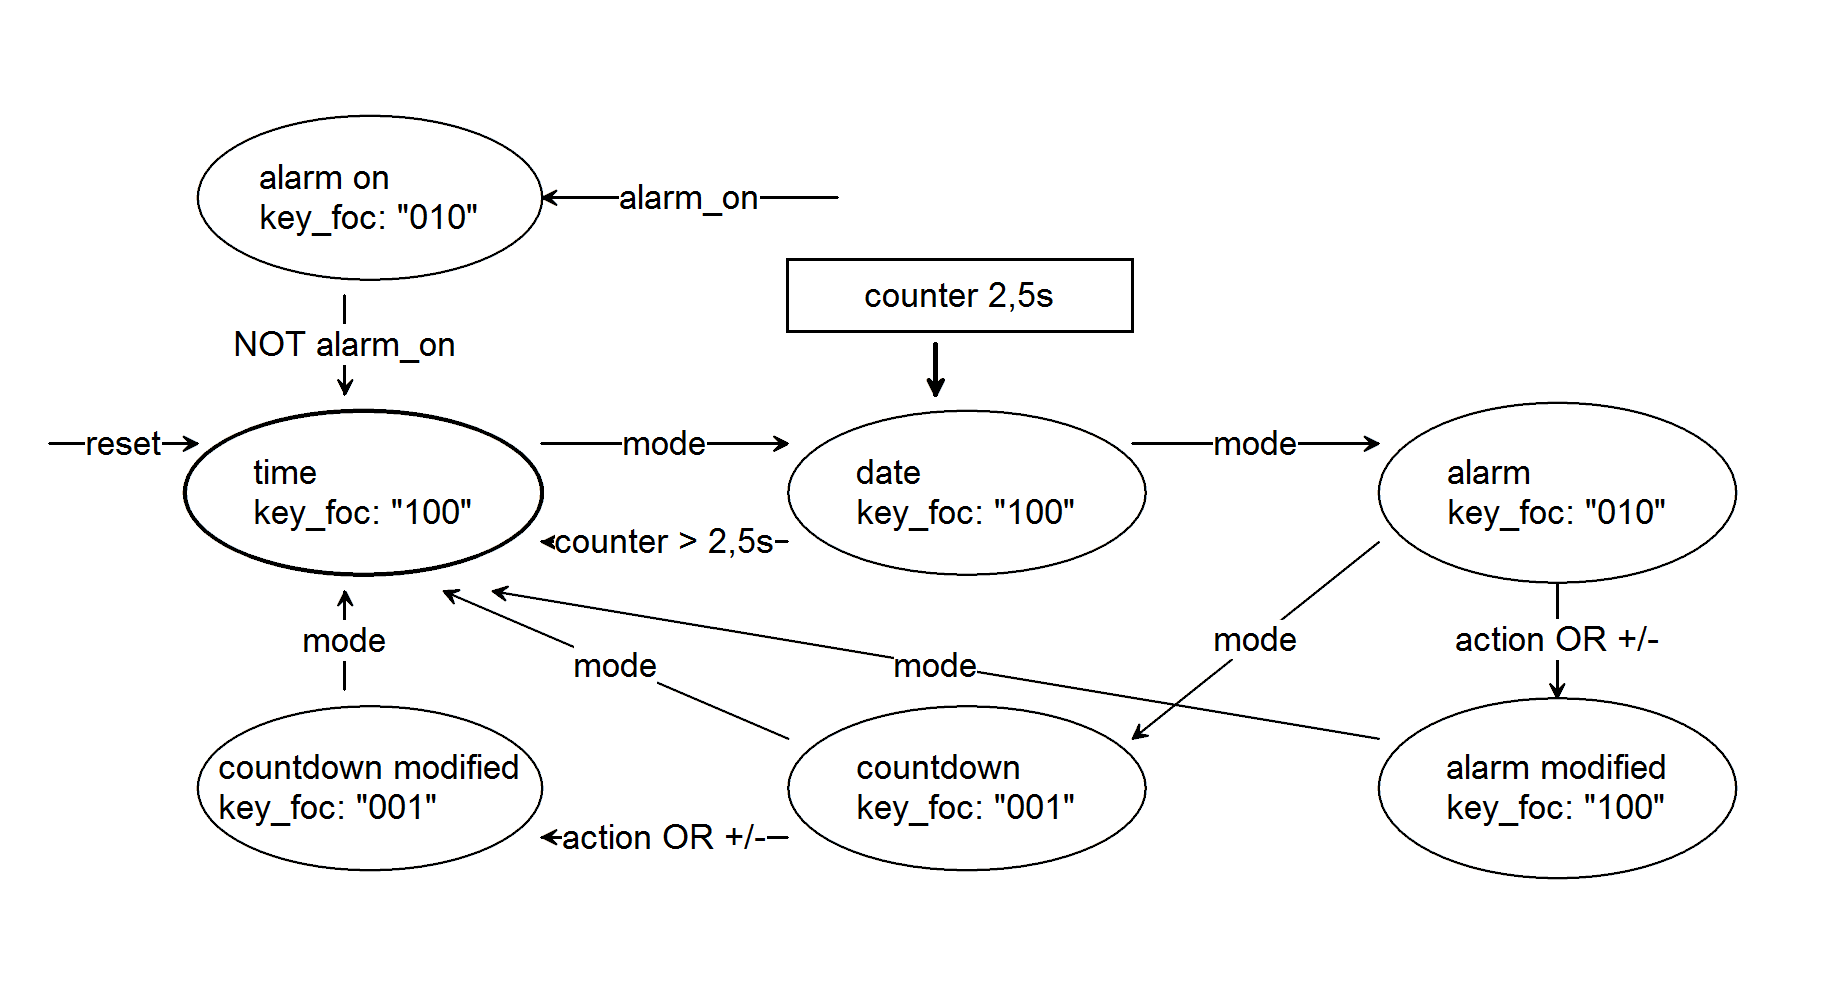
\includegraphics[width=100mm, height=70mm]{mode_fsm_state.png}
    \end{figure}
  \end{frame}



\begin{frame}{Display\_mux Interface}
    \begin{columns}
    \begin{column}{6cm}
        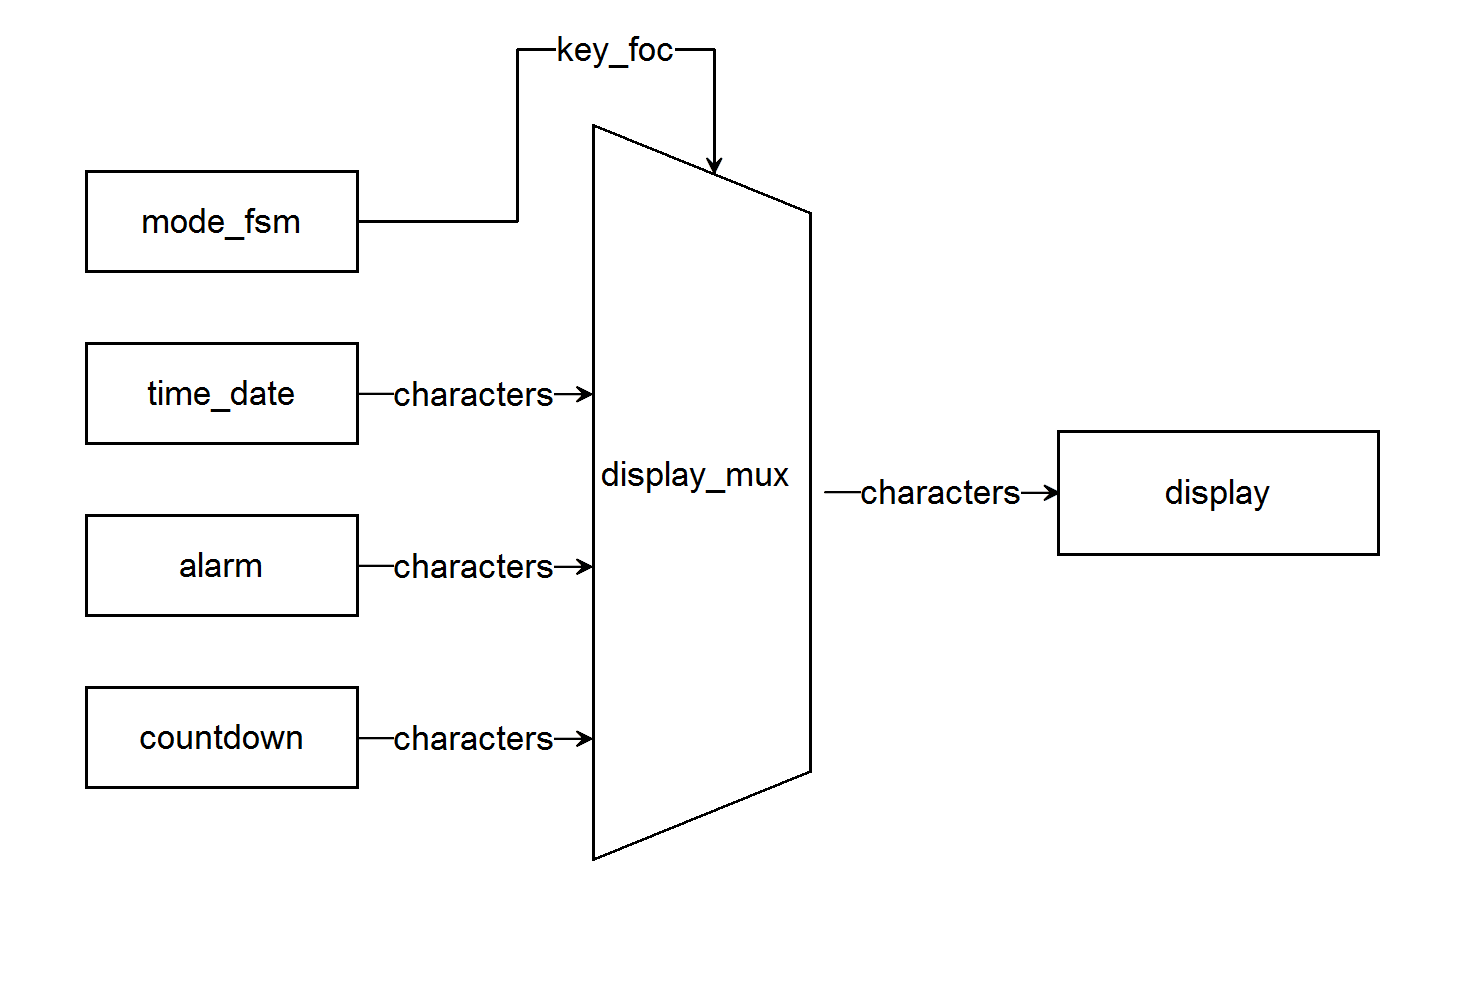
\includegraphics[width=60mm, height=50mm]{display_mux_interface.png}
    \end{column}
    \begin{column}{6cm}
    \begin{itemize}
        \item forwards characters of aktive module
        \item "DCF" string and star for active alarm always from time\_date/alarm module 
    \end {itemize}
    \end{column}
    \end{columns}
  \end{frame}
\end{document}

